%!TEX root = ../DeGaulle.tex
\section{Conclusions}

	In the present paper an original approach to doing calculations on different levels of isotopic fine structure aggregation hierarchy was proposed. To our best knowledge, it is the first use of Poisson approximation for algorithmic purposes,   resulting already in two elegant algorithms, \textsc{DeFine} and \textsc{DeFiner}, for efficient exploration of the state space of possible isotopic configurations.  

	\textsc{DeFine} presents a minimalistic, yet extremely efficient way to calculate the approximate probabilities of {\it equatransneutronic} clusters. \textsc{DeFiner} presents a simple, yet certainly suboptimal way of handing Problem \ref{Problem of finding LFS_K configurations.}; however, more efficient algorithms can easily come into being by more careful considerations on the structure of approximative distribution $\QK$. 

	Figure \ref{figure: hierarchy} presents a detailed view of the hierarchical approach we take. The left pane contains the  aggregated isotopic distribution of \testAvergine, an $100$-avergine, obtained with the {\sc BRAIN} algorithm \cite{Dittwald2013BRAIN}. The lower panel zooms into the region of the highest aggregated peak. This peak is then disaggregated into {\it equatransneutronic} groupings. Finally, one notices many small black peaks corresponding to the finest structure obtainable. It is by clustering and statistical centroiding of these peaks that one obtains all the others. 

\begin{figure}[htbp]
 \centering
 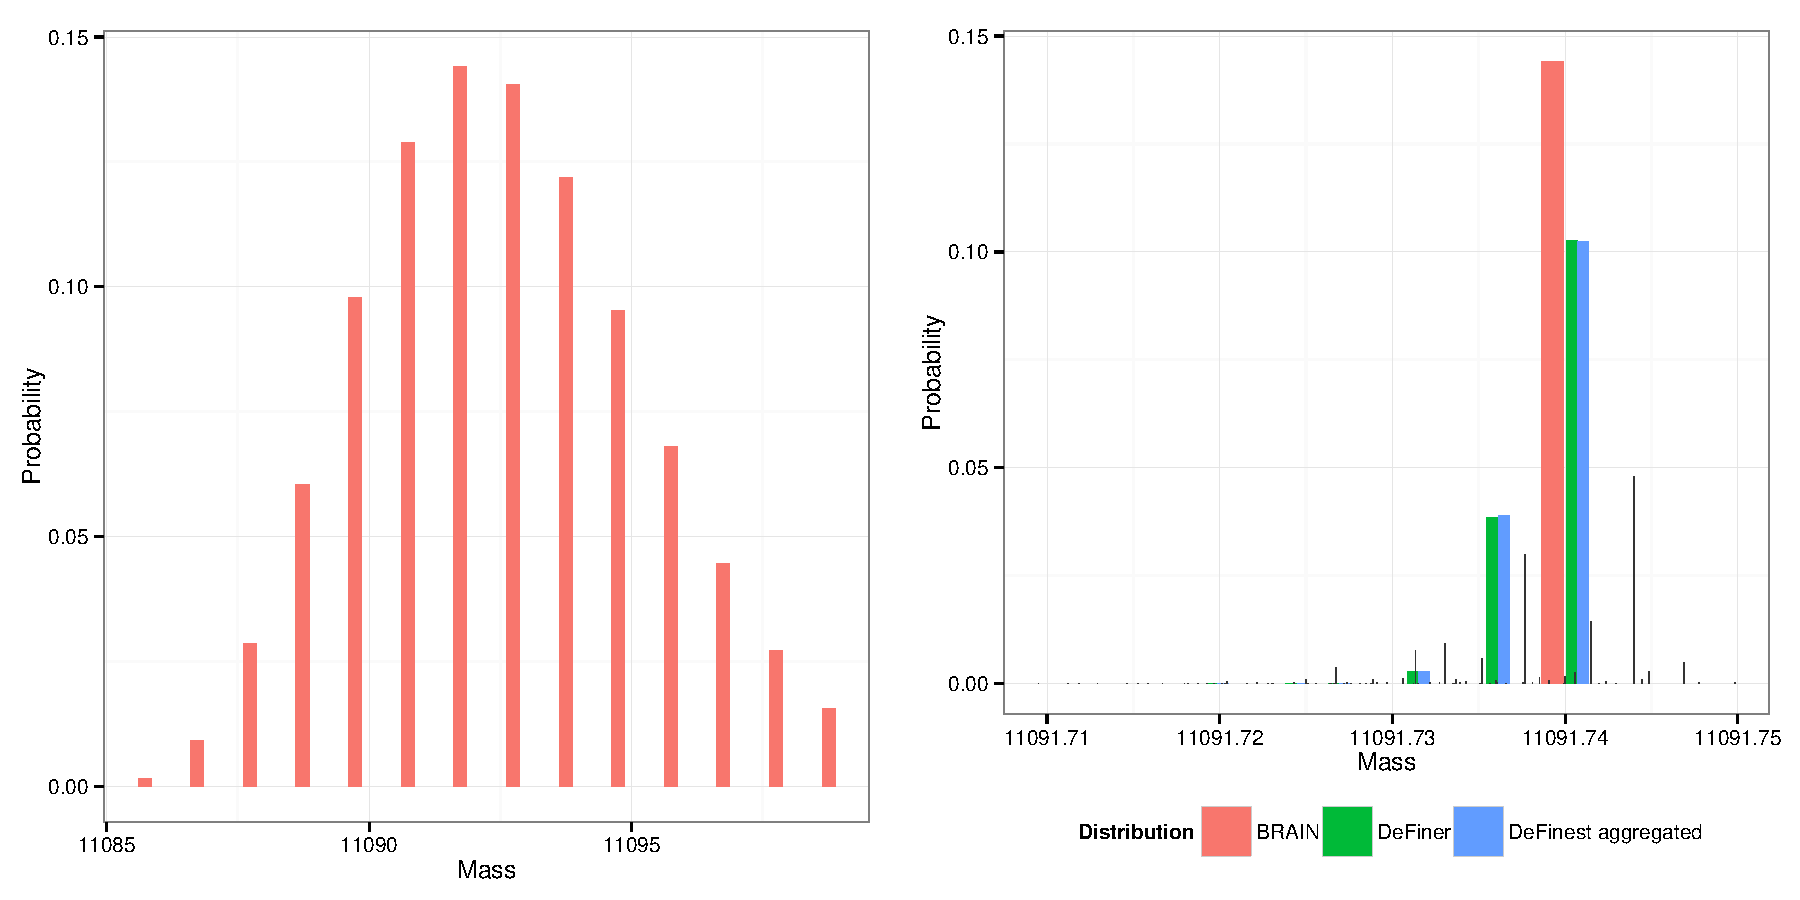
\includegraphics[width=\textwidth]{./img/hierarchyHorizontal}
 \caption{ Peaks in the left pane are probabilities of different $LFS_K$ groups, $K = 0,\dots,13$. In the right pane masses of configurations in $LFS_6$ are plotted: it zooms the region around the tallest peak in the left pane, which is also plotted there for reference. By appropriately aggregating \textsc{DeFiner}'s results, i.e. small black peaks, we calculate the {\it equatransneutronic} precise, non-approximated probabilities, in blue. We compare them with \textsc{DeFine}'s results obtained {\it via} the Poisson approximation, in green. There are no apparent differences between them. }
 \label{figure: hierarchy}
\end{figure}


	The potential applications of our results are numerous. Above all, the fine structure models can find application in automatic top-down peptide identification procedures by establishing more detailed fingerprints thereof and possibly boosting the ability to differentiate between similar compounds. Differences in the fine structure with $K^*$ s.t. $\mathbb{M}_{K^*}(LSF_{K^*}) = \max_K \MK(LSF_K)$ could be particularly informative.


	As another application, one can ask how to set up an optimal binning procedure. Simply, with a critical set of configurations $A$, s.t. $\MK(A) \approx 95\%$, how should these configurations be glued together to match real data from a mass spectrometer. This way, one could measure the machine's resolution without a need to refer to somewhat underdefined notions of {\it p percent valley} and {\it peak width}, see \cite{Eidhammer2008ComputationalMethodsInMassSpectrometry}. 


	Observe that in this article we do not comment on the quality of the approximations in use. The reason behind it is that to our best knowledge no-one has ever carried out a thorough statistical research comparing which of these distributions is better suited for modelling the actual data. From the theoretical perspective, it seems plausible to adopt the most simple model of the isotopic fine structure probability, $\MM$, as developed in \cite{Kienitz1961MassSpectrometry}. However, with $\QQ$ at hand, and many data sets at disposal, one could verify whether such hypothesis holds. To our best knowledge, up to this moment only comparisons between theoretical distributions were carried out \cite{Valkenborg2007UsingPoisson}. We are of opinion that only through comparisons explicitly based on empirical data should one decide on the quality of the two models.



	% Moreover, at least in case of {\it Time of Flight} analyzers, there is an additional advantage of studying the {\it localised fine structure}, for their resolution is a function of the mass of analyte, see \cite{Eidhammer2008ComputationalMethodsInMassSpectrometry}. It is more difficult to differentiate correctly between molecules with similar masses, when both of them are big. 


	% However, we judge that all such algorithms could share the idea of using, in one way or another, the approach developed in {\sc Define}: namely, start by choosing a configuration presumed to be in vicinity of the mode of $\MK$, and proceed by a controled {\it breadth first search} until either a certain number of configurations is reached, or they already gathered ones already have enough of probability upon them.

	% A different problem to those mentioned before could be solved in this way to, namely:  

	% \begin{Problem}\label{Big Problem}
	% 	Find a small set $C$ among all possible configurations, s.t. $\mathbb{M}(C) \approx 1$.
	% \end{Problem}

	% The candidate for the biggest peak would by then be the product of modes of each multinomial model in \eqref{product of multinomials}.

	% This problem has been more efficiently be solved by different approaches, e.g. by the use of Fourier transform methods, see \todo{Find Rockwood's publication.}. 



	% Models solving Problem \ref{Big Problem} would have to add some sort of binning procedure with bin width being a function of mass, that not being straightforward to model. Thanks to the localisation in the mass to charge domain, while studying $LFS_K$ we simply neglect that sort of problem.